\documentclass[preprint,12pt]{elsarticle}

% --------------------------------------------------
% Packages required by the current manuscript
% --------------------------------------------------
\usepackage{amsmath}
\usepackage{graphicx}
\usepackage{booktabs}
\usepackage{tabularx}
\usepackage{graphicx}
\usepackage{booktabs}
\usepackage{tabularx}
\usepackage{array}
\usepackage{makecell}
\usepackage{multirow}
\usepackage{xcolor}
\usepackage[hidelinks]{hyperref}   % url handling; makes \url{...} accept
                                    % underscores in bib entries and turns
                                    % references clickable in the PDF.

% --------------------------------------------------------------
% DRAFT-ONLY ANNOTATIONS
% One switch controls every draft annotation: the pre-submission task
% list after the front matter and all inline [TODO] markers. Flip it
% to \showtasksfalse for a clean submission PDF.
% --------------------------------------------------------------
\newif\ifshowtasks
\showtasksfalse         % <-- set to \showtaskstrue while drafting

\newcommand{\TODO}[1]{\ifshowtasks\textcolor{red}{\textbf{[TODO: #1]}}\fi}

% --------------------------------------------------
% Document
% --------------------------------------------------
\begin{document}

\begin{frontmatter}

\title{Association Between Adherence to Inpatient Diabetes Care Guidelines
and Hospitalization Complications: A Multicenter Real-World Study}

% --------------------------------------------------
% Authors
% --------------------------------------------------
\author[aff1]{Shahar Oded}
\author[aff1]{Yuval Shahar}
\author[aff1]{Erez Shalom}
\author[aff2,aff3]{Amir Bashkin}
\author[aff4,aff5]{Leonard Saiegh}
\author[aff6]{Dror Cantrell}
\author[aff7]{Irit Wirsansky}
\author[aff2,aff8]{Muhamad Badarne}
\author[aff9]{Irena Barash}
\author[aff10,aff11]{Avivit Cahn}
\author[aff4,aff7]{Irit Hochberg}

% --------------------------------------------------
% Affiliations
% --------------------------------------------------
\address[aff1]{Medical Informatics Research Center,
Ben-Gurion University of the Negev, Beer Sheva, Israel}

\address[aff2]{Azrieli Faculty of Medicine,
Bar-Ilan University, Safed, Israel}

\address[aff3]{Endocrinology and Diabetes Unit,
Galilee Medical Center, Nahariya, Israel}

\address[aff4]{Bruce Rappaport Faculty of Medicine,
Technion--Israel Institute of Technology, Haifa, Israel}

\address[aff5]{Endocrinology Institute,
Bnai Zion Medical Center, Haifa, Israel}

\address[aff6]{Internal Medicine Department C,
Shamir Medical Center, Beer Yaakov, Israel}

\address[aff7]{Endocrinology Unit,
Hillel Yaffe Medical Center, Hadera, Israel}

\address[aff8]{Endocrinology and Diabetes Service,
Tzafon Medical Center, Ramat Poriya, Israel}

\address[aff9]{Internal Medicine Department C,
Barzilai Medical Center, Ashkelon, Israel}

\address[aff10]{Internal Medicine Department A,
Hadassah Ein Kerem, Jerusalem, Israel}

\address[aff11]{Faculty of Medicine,
Hadassah Hebrew University Hospital, Jerusalem, Israel}

% --------------------------------------------------
% Abstract
% --------------------------------------------------
\begin{abstract}

\textbf{Objective:}
To measure adherence to a national inpatient hyperglycemia guideline at the
level of its individual recommendations across a hospital network, to
determine whether adherence changed following the guideline's introduction,
and to identify which recommendations are associated with subsequent
clinical outcomes.

\textbf{Methods:}
Retrospective multicenter study of 48,354 admissions among 29,577 adult
patients with diabetes or inpatient hyperglycemia across six Israeli general
hospitals, August 2022 to December 2025. Each of fourteen guideline
recommendations was formalized as a quality-assessment temporal pattern over
knowledge-based temporal abstractions of the clinical record, yielding a
continuous compliance score wherever the recommendation applied. Adherence
before and after the guideline's introduction was compared using Welch's
$t$-test with false discovery rate correction. Associations with ten
complications were estimated by bias-reduced logistic regression over 24-,
48-, and 72-hour observation windows, and by inverse probability of
treatment weighting contrasting above- with at-or-below-median adherence.

\textbf{Results:}
Adherence varied widely across recommendations, from near-universal
implementation of admission and medication-management actions to substantial
gaps in insulin management (mean scores $0.15$--$0.28$).
Overall adherence increased modestly after the guideline was issued
($0.682$ to $0.703$, $p<0.001$), with substantial inter-hospital
heterogeneity. After propensity weighting, above-median adherence was
associated with lower odds of 30-day mortality (OR $=0.557$, 95\% CI
$[0.514, 0.603]$), hyperglycemia (OR $=0.175$, 82.5\% lower odds) and severe hyperglycemia
(OR $=0.485$), and with a modest increase in hypoglycemia (OR $=1.204$, 20.4\% higher odds). 
The association with severe hypoglycemia was directionally consistent but
not significant. At the component level, routine basal insulin dosing,
routine glucose monitoring, and insulin administration following
hyperglycemia remained associated with lower mortality.

\textbf{Conclusion:}
Guideline adherence can be assessed automatically and per-recommendation at
the scale of a national implementation. The recommendations least well
implemented were largely those whose adherence tracked subsequent outcomes:
the repeated insulin decisions distributed across a
hospitalization, rather than the discrete actions taken on admission. These
associations are not treatment effects, but they identify where fuller
implementation would most plausibly matter.

\end{abstract}

% JBI permits 1--7 keywords.
\begin{keyword}
inpatient diabetes
\sep clinical guideline adherence
\sep quality assessment
\sep temporal abstraction
\sep fuzzy logic
\sep propensity score
\sep causal inference
\end{keyword}

\end{frontmatter}

% --------------------------------------------------
% Draft-only task list (suppressed by \showtasksfalse; not part of the
% manuscript). Guarded, so the manuscript still compiles wherever this
% draft-only file is absent -- e.g. a submission upload that omits it.
% --------------------------------------------------
\IfFileExists{tasks.tex}{% =====================================================================
% DRAFT-ONLY: pre-submission task list.
%
% Rendered only while \showtaskstrue is set in main.tex. Carries no
% manuscript content. Flipping the switch to \showtasksfalse removes
% this box and every inline [TODO] marker at once.
%
% Kept identical to JAMIA2027/tasks.tex -- the two manuscripts share
% these open items, so update both together.
% =====================================================================
\ifshowtasks
\begin{center}
\fcolorbox{red}{red!4}{%
\begin{minipage}{0.94\textwidth}
\vspace{2pt}
\textcolor{red}{\textbf{DRAFT --- OPEN TASKS BEFORE SUBMISSION}}
\vspace{4pt}
\hrule
\vspace{6pt}
\footnotesize
\begin{enumerate}\setlength{\itemsep}{5pt}\setlength{\parskip}{0pt}

\item \textbf{Funding statement.} Name the funding body and grant number,
or state that the work received no specific grant. Elsevier expects the
exact wording ``This research did not receive any specific grant from
funding agencies in the public, commercial, or not-for-profit sectors''
where that applies. \emph{(Section: Funding.)}

\item \textbf{Export the curated concept indices from the closed
environment.} The manuscript now states that the indices are provided as
supplementary material (Methods and the Data Availability statement both
say so). That claim is not yet true --- the files must be exported from
the hospital VM and attached before submission, or both statements must
be walked back.

\end{enumerate}
\vspace{4pt}
\end{minipage}}
\end{center}
\vspace{6pt}
\fi
}{}

% --------------------------------------------------
% Main manuscript
% --------------------------------------------------
% introduction.tex already begins with \section{Introduction}
\section{Introduction}
\label{sec:introduction}

Diabetes mellitus affects approximately 537 million adults worldwide, a
figure projected to reach 783 million by 2045
\citep{idf-atlas-10th-edition-2021}. In Israel, the national diabetes
registry documents a steadily growing patient population over the past
decade
\citep{israel-national-center-disease-control-diabetes-registry-report-2012-2022},
with a corresponding burden on the health system
\citep{summary-cost-diabetes-israel-2018}. That burden is concentrated in
hospital care: approximately 40\% of patients admitted to Israeli general
hospitals have diabetes \citep{hochberg2023inpatient}.

In hospital the clinically relevant object is not the diagnosis but the
glycemic state during the admission. Hyperglycemia arising in hospital is
associated with infection, delayed healing, metabolic decompensation and
increased mortality, and occurs in patients with and without documented
diabetes. Its counterpart, hypoglycemia, is acute, harmful, and largely
iatrogenic---a consequence of the insulin used to correct the first problem.
Inpatient glycemic management is therefore a balancing act shaped less by any
single decision than by how monitoring, medication management and insulin
dosing are carried out repeatedly across a stay. That makes the treatment
process itself, not only the patient's state, worth measuring.

Guidelines exist to standardize such processes. In September 2023 the Israel
Endocrine Society, the Israel Diabetes Association and the National Diabetes
Council issued a national position paper on inpatient diabetes care
\citep{hochberg2023inpatient}, specifying how often glucose should be
measured, how oral antidiabetic agents should be handled on admission, when
basal and correction insulin should be given, and how to respond to
hyperglycemic and hypoglycemic episodes. Recommendations of this kind are
checkable in principle because they are procedural, temporal and
conditional: an action is expected, within some window or at some frequency,
when a triggering situation holds.

Establishing whether they were followed is harder. Guidelines are published
as text, must be adapted to the individual patient, and are known to be
applied incompletely. Retrospective assessment has conventionally required
chart review, which does not scale past modest single-institution
samples---too small to separate one ward's practice from the effect of a
guideline, and far too small to see how practice shifts when a guideline is
introduced nationally. The question that matters most to a guideline's
authors is therefore rarely answerable: not whether the guideline is sound,
but which of its individual recommendations are adopted, and which of them
measurably change what happens to patients.

This study addresses that question. Each recommendation was formalized as a
temporal pattern over abstracted clinical data, using knowledge-based
temporal abstraction \citep{shahar1997framework} and the quality-assessment
formulation of adherence \citep{ben2024supporting}, producing a continuous
compliance score automatically wherever the recommendation applies. Applying
this to 48,354 admissions across six general hospitals spanning the
guideline's introduction, we ask how completely each recommendation was
implemented and whether that changed after issue; whether adherence is
associated with subsequent outcomes once measured patient characteristics
are accounted for; and which individual recommendations carry that
association. Adherence thus serves as an explanatory variable, and the
guideline's recommendations as hypotheses to be tested against what
subsequently happened to the patient.

% JBI requires a Statement of Significance at the end of the Introduction.
\begin{table}[h]
\centering
\caption{Statement of Significance}
\label{tab:significance}
\begin{tabularx}{\textwidth}{
>{\raggedright\arraybackslash}p{0.22\textwidth}
>{\raggedright\arraybackslash}X
}
\toprule

\textbf{Problem} &
Adherence to inpatient diabetes guidelines is known to be incomplete, but
assessing it retrospectively has required manual chart review. This does not
scale to the size needed to distinguish local practice from the effect of a
guideline, or to observe how practice changes when one is introduced
nationally. \\

\midrule

\textbf{What is Already Known} &
Knowledge-based temporal abstraction and quality-assessment temporal
patterns allow guideline adherence to be scored automatically from clinical
records, and have been demonstrated in single-institution settings. Prior
applications evaluate care \emph{against} the guideline, which serves as the
reference standard. \\

\midrule

\textbf{What This Paper Adds} &
An automated, component-level assessment of a national inpatient
hyperglycemia guideline across six hospitals and 48,354 admissions spanning
its introduction, together with a transferable knowledge base encoding it.
By treating each recommendation as a testable hypothesis rather than as a
fixed standard, the study identifies which recommendations were least
implemented and which are associated with subsequent outcomes---and finds
these to be largely the same set. \\

\bottomrule
\end{tabularx}
\end{table}


% related_work.tex already begins with \section{Related Work}
\section{Related Work}
\label{sec:related-work}

The work reviewed here forms one continuous line of research, running from
the representation of clinical concepts, through the machine-interpretable
representation of clinical guidelines, to the retrospective assessment of
whether those guidelines were followed. It supplies both the abstraction
layer and the adherence measure used here, beginning with knowledge-based
temporal abstraction and the Temporal Mediator
\citep{shahar1997framework}---the framework that turns time-stamped clinical
data into named interval concepts, and the engine that executes a knowledge
base against a patient record to derive them.

Formalizing a guideline requires two kinds of knowledge: \emph{declarative}
knowledge, defining what its terms mean, and \emph{procedural} knowledge,
specifying what to do and when. Asbru
\citep{shahar1997asbru, shahar1998asgaard} is the language in which the
procedural half is conventionally expressed, representing sequential,
concurrent, conditional and repetitive actions as a hierarchy of execution
plans.

Picard
\citep{shalom2016architecture}
combines declarative knowledge executed by the Mediator with procedural
knowledge in Asbru to generate real-time recommendations, adherence reports,
and alerts for critical deviations. It served as the decision-support engine
of the MobiGuide project
\citep{peleg2022mobiguide},
which supported chronic disease management in Spain and Italy; there, the
engine improved clinicians' compliance with guidelines from 41\% in manual
mode to 93\%---direct evidence that adherence is malleable, and therefore
worth measuring.

Retrospective assessment required a third body of knowledge.
\emph{Quality-assessment} knowledge \citep{ben2024supporting} re-expresses a
guideline's procedural content declaratively, as the temporal pattern its
correct execution would have left in the record---a quality-assessment
temporal pattern. Acquiring it is a knowledge-engineering task in itself:
each recommendation must be classified by the constraint it imposes and given
a membership function grading partial compliance rather than a binary
verdict. Such systems are conventionally evaluated for the correctness and
completeness of their recommendations, first against simulated scenarios and
then silently on real data \citep{shalom2015multiple}. The assessment
machinery has also been applied institutionally: a system for long-term
management at a geriatric hospital \citep{shalom2024implementation} showed
that automated assessment recovers clinically meaningful variation in how
protocols are followed.

The present study adopts this formulation of adherence, but not the systems
that introduced it. No recommendations are produced and no decision-support
engine is deployed; scoring is performed offline, over records already
collected. Three differences position the work. In \emph{representation},
rather than maintaining a procedural formalism alongside a declarative one,
both are encoded in a single schema evaluated by one engine, and the
knowledge base itself---formalizing the national inpatient diabetes
guidelines together with their quality-assessment extension---is a
contribution transferable to any electronic health record within that
clinical scope. In \emph{scale}, prior assessments have generally been
confined to modest cohorts within a single institution, which can separate
neither the practice of a particular ward from the effect of a guideline,
nor observe how practice shifts when a guideline is introduced nationally;
here adherence is measured across six hospitals spanning such an
implementation. In \emph{purpose}, these systems are evaluated \emph{against}
the guideline, which serves as the yardstick and whose clinical value is
inherited from the research establishing it. This study encodes the same
predetermined guideline, but treats its individual recommendations as
hypotheses to be tested against what subsequently happens to the patient.
Adherence thus serves as an explanatory variable rather than only as the
quantity reported: the question is not whether the guideline was applied
correctly, but which of its recommendations demonstrably matter.


% methods.tex already begins with \section{Methods}
\section{Methods}
\label{sec:methods}

\subsection{Study Design and Data Source}

We conducted a retrospective multicenter study using electronic health
record data from six Israeli general hospitals, drawn from Kineret
\citep{rappoport2025kineret}, the
data warehouse of Israel's largest hospital network, represented in the
Observational Medical Outcomes Partnership (OMOP) common data model. Data
were extracted in two batches corresponding to the periods before and after
the national implementation of the inpatient hyperglycemia-treatment
recommendations. The analysis window spanned August 2022 through December
2025.

The assessed recommendations are those of the national position paper on
the treatment of diabetes in hospitalization in a general hospital
\citep{hochberg2023inpatient}, issued in September 2023 by the Israel
Endocrine Society, the Israel Diabetes Association, and the National
Diabetes Council. The pre-intervention period therefore ends immediately
before its publication and the post-intervention period begins a year after
it, with the intervening months excluded to allow for staggered adoption.

The study received Helsinki committee approval covering up to 30,000 adult
patients admitted between 2022 and 2025, defined by the cohort criteria set
out in Section~\ref{sec:cohort-definition}.

\subsection{From OMOP Tables to a Unified Event Dataset}

The source OMOP tables were reorganized into five unified, columnar
tables---visits, visit types, clinical events, drug exposures, and
measurements---without semantic transformation. Measurement units were
normalized at this stage, but source concept identifiers and names were
preserved verbatim, so that all terminology decisions are made explicitly at
the abstraction stage rather than being embedded in the extract.

Kineret was not mapped to an international coding system at the time of this
work, so a dataset-specific concept index---a many-to-one mapping from local
measurement, medication, and observation codes onto the concepts named in
the knowledge base---had to be constructed before abstraction could proceed.
The index is what makes the remainder of the pipeline dataset-agnostic: once
it exists, the same knowledge base and engine run unchanged on any source
within the same clinical scope. Curation was performed jointly by a clinical
domain expert and a data scientist, with candidate codes surfaced by
descriptive analytics over the extracted concept dimensions and adjudicated
by the domain expert. The curated indices, rather than the exploratory
analytics used to generate the candidate lists, are the reproducible
artifact of this step, and are provided as supplementary material.
Further detail on the extraction and on the derived concepts is given in
Appendix~\ref{app:data-prep}.

\subsection{Cohort Definition}
\label{sec:cohort-definition}

An admission was considered eligible if it satisfied all of the following
conditions. The admission was an inpatient visit with at least one
measurement recorded between 18:00 and 07:00, used as evidence of a genuine
overnight stay; its length of stay was between 48 hours and 14 days; the
patient was at least 18 years old at admission; the admission did not take
place in an excluded department; the visit identifier was not associated
with more than one patient identifier, which was treated as a data-integrity
failure; the patient did not die within 48 hours of admission; and the
admission met at least one criterion for diabetes or hyperglycemia.

Exclusions were applied through curated indices rather than inline rules, so
that each exclusion is recorded once alongside the concept vocabulary and
applied uniformly across the pipeline. Pediatric and obstetric departments
were excluded, which together with the adult age criterion also removes
pregnancy-related admissions, including gestational diabetes.

Diabetes or hyperglycemia was established by at least one of three
non-mutually-exclusive criteria: (i) a documented diabetes diagnosis,
identified through a manually curated list of concept identifiers;
(ii) recurrent hyperglycemia, defined as two glucose measurements
$\geq180$ mg/dL separated by at least 2 and at most 24 hours; or
(iii) extreme hyperglycemia, defined as any glucose measurement
$\geq250$ mg/dL. Hypoglycemia was deliberately not used as an entry
criterion: the cohort is defined by hyperglycemic burden, and hypoglycemia
is treated throughout as an outcome rather than as a route into the study
population.

For the pre--post comparison, admissions between August 2022 and July 2023
constituted the pre-intervention period and admissions between August 2024
and December 2025 the post-intervention period. The intervening months were
excluded from the primary comparison to allow for staggered adoption.

Thirty-day mortality was defined from the linked death records as death
occurring between 14 days before and 30 days after the recorded discharge
datetime. The backward tolerance accommodates admissions in which the death
record precedes the administrative discharge timestamp, so that in-hospital
deaths are captured.

\subsection{Constructing the Abstraction Input}

Two inputs were derived from the unified event dataset.

The \emph{temporal input} is a long-format table in which each row records a
single time-stamped clinical fact: admission identifier, concept name, start
and end datetime, and value. A small number of concepts were derived rather
than extracted directly, and structural tokens were inserted to make the
admission timeline explicit to the abstraction engine---an \textsc{admission}
token at the visit start, a terminal \textsc{release} or \textsc{death}
token at its end, and recurring \textsc{meal} tokens at fixed daily times,
which supply the anchors required by recommendations defined relative to
meals. Meal times are not recorded in the source data and were therefore
assumed to occur at fixed daily times---breakfast, lunch, dinner, and a
night snack---following standard hospital practice. Selected concepts
recorded before admission, such as chronic
diagnoses and home medications, were propagated into the admission window
using per-concept relevancy lookback periods
(Appendix~\ref{app:data-prep}).

The \emph{context input} is a static table with one row per admission,
holding baseline characteristics ascertained from the first 48 hours:
demographics, chronic condition flags, and indicators distinguishing
medications taken at home from those administered in hospital. From these
flags a comorbidity score was computed, following the structure of the
Charlson Comorbidity Index and referred to throughout as a modified Charlson
comorbidity index (CCI). The modification was necessary because the source
dataset was not mapped to a standard vocabulary, so condition categories
were available only to the extent that the corresponding codes could be
identified during curation; the weighting was adapted to the categories the
extract supports, and is given in Appendix~\ref{app:data-prep}.

\subsection{Guideline Adherence Assessment}

Guideline adherence was assessed by knowledge-based temporal abstraction
\citep{shahar1997framework}, which converts time-stamped clinical data into
named interval concepts---states, trends, events, and contexts---and then
detects, over those intervals, the temporal pattern that correct execution
of each recommendation would have left in the record
\citep{ben2024supporting}. Abstraction and
assessment are performed by the Temporal Mediator in a single pass, using
our reimplementation of it \citep{mediator-github}. All domain knowledge is
declared externally as XML units validated against a shared schema, so that
both the clinical semantics and the guideline requirements are stated once,
outside the analysis code.

Each recommendation is formalized as a quality-assessment temporal pattern:
an \emph{anchor} identifying the clinical situation in which the
recommendation applies, an \emph{action} that satisfies it, a constraint
type, and a membership function grading partial compliance. Applicability is
enforced by context---an anchor falling outside the context in which the
recommendation holds generates no obligation and is not scored---so that
an insulin dose after a meal, for example, is required only
where glucose levels are elevated. Recurring recommendations such as routine glucose
monitoring are instead evaluated by counting qualifying events within
fixed-length windows across the admission.

Compliance is graded rather than binary. Each constraint carries a
trapezoidal membership function mapping the observed timing, frequency, or
value to $[0,1]$: if correction insulin is expected within 4 hours of a
hyperglycemic reading and considered missed after 12, insulin given at 8
hours scores $0.5$ rather than counting as an outright failure. Three
constraint types are used, corresponding to the compliance aspects reported
in the Results---\emph{time}, the interval between anchor and action;
\emph{value}, the magnitude of the recorded value, most often a dose; and
\emph{cyclic}, the number of qualifying events within a window. Aspect
scores are computed separately and averaged at analysis, and trapezoid
boundaries may be rescaled per patient, which is how weight-normalized
dosing is expressed.

Two conventions govern unmet obligations. Where the recommendation requires
an action, an unanswered anchor scores 0; where it requires an action to be
withheld, the absence of a response is itself compliant and scores 1. A
recommendation that never became applicable yields no output rather than a
zero, so inapplicable recommendations do not depress the score.

Discretization thresholds, relevance durations, and trend limits were
acquired in two passes. One-dimensional $k$-means and kernel density
estimation over each concept's value distribution proposed candidate
boundaries; these were then reconciled against published reference ranges
and the definitions in the national guideline, which were authoritative,
with the data-driven candidates used only to resolve cases where the
literature gives a range rather than a value. Concepts with too many
distinct value combinations for in-engine discretization, such as
corticosteroid preparations at varying doses, were pre-discretized during
data preparation.

The knowledge base was authored by the first author and developed under the
guidance of two co-authors, one specializing in medical informatics and
temporal reasoning and one in diabetes care, who reviewed the formalized
recommendations for clinical fidelity against the source position paper
\citep{hochberg2023inpatient}. Because it names clinical concepts
rather than dataset columns, it is transferable to any electronic health
record within the same clinical scope once a concept index maps that
source's codes onto its vocabulary. Scoring is retrospective and offline:
the procedure issues no recommendation and returns nothing to the treating
team. The engine emits one compliance score per admission, pattern,
compliance aspect, and evaluation time, and these scores are the exposure
variable for all subsequent analyses.

\subsection{Outcome Definitions}

Ten complications were evaluated: 30-day mortality, hyperglycemia, severe
hyperglycemia, hypoglycemia, severe hypoglycemia, hyperosmolality,
ketoacidosis, infection, Inpatient acute kidney injury (AKI), and inpatient myocardial infarction (MI).
All ten are emitted as abstractions by the same engine, so that outcome
ascertainment and adherence assessment draw on a single, explicit knowledge
base. They differ only in where the underlying logic is evaluated. The
glycemic outcomes and acute kidney injury are derived by the engine directly
from measurements: hyperglycemia and hypoglycemia from glucose values, using
a parameterized concept that distinguishes a sustained state from an
isolated reading, and acute kidney injury from serum creatinine and its
ratio to baseline. Ketoacidosis, infection, hyperosmolality, and myocardial
infarction require multi-step logic combining several concept types with
their own temporal windows, and were therefore precomputed during data
preparation and supplied to the engine as primitive concepts, which it
re-emits as complication events. Thirty-day mortality is taken from the
linked death records.

Two outcomes are reported under abbreviated labels and warrant note here.
MI requires evidence of an ischemic
cardiac event together with a troponin level of at least 600, so that coded
cardiac history unaccompanied by biochemical evidence of acute injury does
not qualify. AKI is defined from laboratory
values as stage 2 or above, excluding stage~1. Full operational definitions
of all ten complications are given in Appendix~\ref{app:definitions}, and
the definitions of the assessed guideline recommendations in
Appendix~\ref{app:patterns}.

\subsection{Statistical Analysis}

\subsubsection{Aggregation of adherence scores}

The admission is the unit of analysis throughout. A patient may contribute
several admissions, and patient-level grouping is applied wherever the
statistics require it, as in the clustered standard errors of the mortality
model below. Compliance scores were aggregated in
stages designed so that neither frequently-evaluated patterns nor
frequently-evaluated days dominate the result. Scores were first averaged
within each admission, pattern, compliance aspect, and calendar day; aspects
were then collapsed within each admission, pattern, and day; days were then
collapsed within each admission and pattern; and finally patterns were
averaged with equal weight to give one overall adherence score per
admission. Component-level analyses use the corresponding pattern-level and
aspect-level aggregates.

\subsubsection{Change in adherence following implementation}

Overall and component-level adherence were compared between the pre- and
post-intervention periods using Welch's unequal-variance $t$-test, with each
admission attributed to a period by its admission date. Confidence intervals for the difference in means are Welch
$t$-intervals and are reported unadjusted; $p$-values were adjusted across
the component-level comparisons using the Benjamini--Hochberg false
discovery rate (FDR) procedure. Monthly means are reported with 95\%
confidence intervals derived from the within-month standard error, and the
overall temporal trend is an ordinary least-squares fit to the monthly
means.

\subsubsection{Adherence and 30-day mortality}

Mean whole-admission adherence was compared between admissions ending in
death within 30 days and those not, using Welch's $t$-test. The graded
relationship was then tested by logistic regression on the continuous score,
reported as the odds ratio per $0.1$-point increase; adherence strata appear
in the corresponding figure for display only, with strata under 30
admissions suppressed, and are not the basis of the trend statistic.

The adjusted estimate was a logistic regression on the overall adherence
score with prespecified covariates---age, sex, the modified Charlson
comorbidity index, and hospital as fixed effects---with continuous
predictors standardized, so the odds ratio corresponds to a
one-standard-deviation increase, and standard errors clustered on patient
identity. Both estimates use whole-admission adherence and are reported as
descriptive.

\subsubsection{Component-level models}

To identify which individual recommendations were associated with each
complication, one model was fitted per complication per observation window.
The analysis dataset contains one row per admission and complication,
labelled positive if the complication first occurred at or after the
observation cutoff and negative if it never occurred; admissions in which
the complication occurred \emph{before} the cutoff were excluded, since a
pre-existing condition cannot be attributed to subsequent in-stay care. Both
adherence and baseline covariates were computed only from admission up to
the cutoff, never afterwards. Cutoffs of 24, 48, and 72 hours were used.

Models were fitted by bias-reduced (Firth penalized-likelihood) logistic
regression \citep{firth1993bias}, with adherence and baseline covariates
entered jointly so that each adherence coefficient is estimated holding
measured comorbidity constant. Firth's method was necessary because
unpenalized maximum likelihood failed to converge under separation for most
complications, given the low event counts of several endpoints; the
Jeffreys-prior penalty yields finite estimates and valid Wald inference
without inducing sparsity. Highly correlated predictors were pruned before
fitting and the remainder standardized so coefficients are comparable.
Benjamini--Hochberg FDR correction was applied within each model's own family
of tested predictors, excluding pruned features, which were never tested. A
bootstrap sign-agreement check flagged estimates whose direction was unstable
under resampling. A predictor was considered robust only if it remained
significant with consistent direction across all three windows.

To avoid mechanical circularity, the routine glucose-monitoring component
was excluded from the models for glycemic outcomes, since glucose
measurement is itself the mechanism by which hyperglycemic and hypoglycemic
events are detected.

\subsubsection{Propensity-weighted analysis}

The recurrent components were re-evaluated using inverse probability of
treatment weighting. Adherence was dichotomized at the median of each
outcome's eligible population, so reported coefficients are log-odds ratios
comparing above-median with at-or-below-median adherence, and the
corresponding odds ratio is $\exp(\beta)$. A binary exposure is intrinsic to
this design rather than a simplification: the propensity score is the
probability of belonging to the high-adherence group conditional on baseline
covariates \citep{rosenbaum1983central}, and the standardized mean
differences used to verify balance \citep{austin2009balance} are two-group
contrasts undefined for a continuous exposure. Continuous adherence is
retained in the regression analyses above, making the two designs
complementary: a conditional estimate from regression adjustment and a
balance-verified marginal contrast from weighting.

Propensity scores were estimated by bias-reduced logistic regression on the
baseline covariates, converted to stabilized weights and trimmed at the
first and ninety-ninth percentiles, and weighted logistic regression models
fitted for each outcome. Balance was assessed by the maximum standardized
mean difference after weighting, with $0.10$ required for an estimate to be
interpretable; component--outcome pairs failing this are reported as
non-estimable, since weighting groups that remain dissimilar does not
support the intended contrast.

\subsubsection{Multiplicity}

Benjamini--Hochberg FDR correction \citep{benjamini1995controlling} was
applied within each family of tests:
across component-level pre--post comparisons, across predictors within each
component-level model, and across outcomes within the propensity-weighted
analysis. Confidence intervals are reported unadjusted throughout, so an
interval excluding the null may accompany a non-significant FDR-adjusted
$p$-value.

\subsubsection{Implementation}

All processing and analysis were performed in Python 3.13. The extraction
and cohort-construction pipeline used \texttt{dask} and \texttt{pyarrow}
over Parquet storage, with \texttt{pandas} and \texttt{numpy} for in-memory
operations; the empirical threshold discovery used $k$-means clustering and
kernel density estimation from \texttt{scikit-learn} with peak detection
from \texttt{scipy}.

Guideline adherence was computed using the Mediator abstraction engine
\citep{mediator-github}, which validates the knowledge base against its XML
schema before evaluating the abstractions.

Statistical analysis used \texttt{statsmodels} for the logistic,
propensity-weighted, and Welch comparisons, together with its
Benjamini--Hochberg implementation for multiplicity correction. Bias-reduced
logistic regression was implemented directly, following Firth's iteratively
reweighted least-squares formulation with a Jeffreys-prior penalty, with
standard errors taken from the penalized information matrix; it is released
with the analysis code rather than drawn from a library.



% results.tex already begins with \section{Results}
\section{Results}

\subsection{Study Cohort}

The study cohort comprised 48,354 hospital admissions among 29,577 unique
adult patients who met the predefined clinical cohort criteria across six
Israeli general hospitals during the study period from August 2022 through
December 2025 (Table~\ref{tab:cohort}). Admissions were distributed across
all six participating hospitals, with center-specific sample sizes ranging
from 4,478 to 11,024 admissions.

The study population had a mean age of 71.9 years (median, 73.3), and
54.3\% were male. The median length of stay was 5.55 days. Among relevant
admissions, 35.3\% had a documented diabetes diagnosis, 74.7\% met the
recurrent-hyperglycemia criterion, and 60.2\% had at least one extreme
glucose measurement. Among admissions with a documented diabetes diagnosis,
50.3\% also met the recurrent- or extreme-hyperglycemia criterion.
Conversely, only 21.5\% of admissions meeting a hyperglycemia criterion
had a documented diabetes diagnosis, indicating that a substantial
proportion of the cohort represented clinically significant inpatient
hyperglycemia without a recorded diabetes diagnosis.

The pre-intervention period contributed 21,605 admissions among 17,002
patients, and the post-intervention period 16,182 admissions among 11,201
patients.

% Table 1: Cohort characteristics
\begin{table}[t]
\centering
\caption{Characteristics of the multicenter study cohort.}
\label{tab:cohort}

\begin{tabularx}{\textwidth}{
>{\raggedright\arraybackslash}X
>{\raggedleft\arraybackslash}p{0.34\textwidth}
}
\toprule
Characteristic & Value \\
\midrule

Hospitals & 6 \\
Admissions & 48,354 \\
Unique patients & 29,577 \\
Age, mean (median), years & 71.9 (73.3) \\
Male sex & 54.3\% \\
Length of stay, median, days & 5.55 \\
30-day mortality & 9.58\% \\

\midrule

Documented diabetes diagnosis & 35.3\% \\
Recurrent hyperglycemia & 74.7\% \\
Extreme glucose ($\geq250$ mg/dL) & 60.2\% \\
Hyperglycemia among admissions with diabetes & 50.3\% \\
Diabetes diagnosis among admissions with hyperglycemia & 21.5\% \\

\midrule

Pre-intervention cohort &
\makecell[r]{21,605 admissions\\17,002 patients} \\

Post-intervention cohort &
\makecell[r]{16,182 admissions\\11,201 patients} \\

\bottomrule
\end{tabularx}
\end{table}


\subsection{Guideline Adherence and Changes Following National Implementation}
\label{sec:adherence-results}

\subsubsection{Overall Guideline Adherence}

Adherence varied sharply across recommendations
(Table~\ref{tab:overall-adherence}), and the split followed the kind of
action required rather than its clinical weight. Single discrete actions on
admission were near-universal: SGLT2 discontinuation was complete ($1.00$)
and creatinine measurement almost so ($0.98$). Recommendations calling for
repeated insulin decisions across the stay were not: insulin following hyperglycemia
scored $0.15$, the two routine basal dosing components $0.21$ and $0.23$,
and bolus reduction after hypoglycemia $0.28$---all with a median of zero,
meaning the expected action was absent altogether in most eligible
admissions. Monitoring and admission medication management fell between
these extremes ($0.54$--$0.88$).

Adherence was largely independent of whether diabetes had been formally
documented. Among admissions with hyperglycemia in the first 48 hours, mean
adherence was $0.669$ where a diagnosis was recorded and $0.661$ where it
was not; the difference of $0.008$ reached significance only by virtue of
the sample size.

\begin{table}[t]
\centering
\caption{Overall adherence to assessed inpatient diabetes guideline recommendations
during the study period. Scores range from 0 (non-adherence) to 1 (complete
adherence).}
\label{tab:overall-adherence}

\begin{tabularx}{\textwidth}{
>{\raggedright\arraybackslash}X
l
r
r
}
\toprule
Guideline recommendation & Constraint & Mean & Median \\
\midrule

Admission glucose monitoring
    & Cyclic & 0.85 & 1.00 \\

Routine glucose monitoring
    & Cyclic & 0.88 & 0.98 \\

Glucose monitoring during corticosteroid therapy
    & Cyclic & 0.54 & 0.50 \\

BMI measurement on admission
    & Time & 0.87 & 1.00 \\

Creatinine measurement on admission
    & Time & 0.98 & 1.00 \\

Antidiabetic discontinuation on admission
    & Time & 0.66 & 0.86 \\

SGLT2 discontinuation on admission
    & Time & 1.00 & 1.00 \\

Basal insulin continuation on admission
    & Time & 0.66 & 1.00 \\

Insulin administration after hyperglycemia
    & Time & 0.15 & 0.00 \\

Antidiabetic discontinuation after hypoglycemia
    & Time & 0.89 & 1.00 \\

Basal dose reduction after hypoglycemia
    & Value & 0.87 & 1.00 \\

Bolus dose reduction after hypoglycemia
    & Value & 0.28 & 0.00 \\

Routine basal dosage (frequency)
    & Cyclic & 0.23 & 0.00 \\

Routine basal dosage (dose)
    & Value & 0.21 & 0.00 \\

\bottomrule
\end{tabularx}
\end{table}


\subsubsection{Changes in Adherence Following the Intervention}

Overall adherence rose from $0.682$ before the guideline to $0.703$ after
($p<0.001$; Figure~\ref{fig:adherence-trend}), with monthly scores trending
upward across the period. The absolute change is small, and its significance
reflects the number of admissions rather than the size of the shift.

Component-level changes were uneven (Table~\ref{tab:adherence-change}).
Glucose monitoring improved most: on admission from $0.78$ to $0.93$
($+0.15$), throughout the stay from $0.83$ to $0.94$ ($+0.11$), and during
corticosteroid treatment from $0.51$ to $0.58$ ($+0.07$). Discontinuation of
high-hypoglycemia-risk antidiabetic agents on admission rose from $0.62$ to
$0.75$ ($+0.13$). Gains in the insulin-management components were significant
but marginal ($+0.01$ to $+0.03$), leaving them close to their already low
baselines. Continuation of basal insulin on admission rose slightly but did
not survive correction ($p_{\mathrm{FDR}}=0.054$), nothing changed in dose
reduction after hypoglycemia, and SGLT2 discontinuation was already complete
in both periods.

Center-level trajectories ranged from improvement through no measurable
change to modest decreases, so the pooled increase conceals substantial
inter-hospital heterogeneity.

\begin{table}[t]
\centering
\caption{Changes in adherence to inpatient diabetes guideline recommendations
before and after the national implementation. Confidence intervals are
unadjusted 95\% confidence intervals for the absolute difference in mean
adherence ($\Delta$). Reported $p$-values were adjusted across component-level
comparisons using the Benjamini--Hochberg false discovery rate (FDR)
procedure.}
\label{tab:adherence-change}

\small

\begin{tabularx}{\textwidth}{
>{\raggedright\arraybackslash}X
rrrrr
}
\toprule
Guideline recommendation & Before & After & $\Delta$ & 95\% CI & $p_{\mathrm{FDR}}$ \\
\midrule

Admission glucose monitoring
    & 0.78 & 0.93 & +0.15 & [0.145, 0.154] & $<0.001$ \\

Routine glucose monitoring
    & 0.83 & 0.94 & +0.11 & [0.105, 0.113] & $<0.001$ \\

Glucose monitoring during corticosteroid therapy
    & 0.51 & 0.58 & +0.07 & [0.062, 0.087] & $<0.001$ \\

BMI measurement on admission
    & 0.86 & 0.89 & +0.03 & [0.015, 0.029] & $<0.001$ \\

Creatinine measurement on admission
    & 0.98 & 0.99 & +0.01 & [0.008, 0.014] & $<0.001$ \\

SGLT2 discontinuation on admission
    & 1.00 & 1.00 & 0.00 & -- & -- \\

Antidiabetic discontinuation on admission
    & 0.62 & 0.75 & +0.13 & [0.075, 0.192] & $<0.001$ \\

Basal insulin continuation on admission
    & 0.63 & 0.67 & +0.04 & [0.002, 0.089] & 0.054 \\

Insulin administration after hyperglycemia
    & 0.14 & 0.15 & +0.01 & [0.009, 0.020] & $<0.001$ \\

Antidiabetic discontinuation after hypoglycemia
    & 0.91 & 0.89 & -0.02 & [-0.197, 0.158] & 0.818 \\

Basal dose reduction after hypoglycemia
    & 0.87 & 0.88 & +0.01 & [-0.015, 0.034] & 0.497 \\

Bolus dose reduction after hypoglycemia
    & 0.33 & 0.26 & -0.07 & [-0.158, 0.029] & 0.210 \\

Routine basal dosage (frequency)
    & 0.21 & 0.24 & +0.03 & [0.027, 0.043] & $<0.001$ \\

Routine basal dosage (dose)
    & 0.19 & 0.22 & +0.03 & [0.021, 0.036] & $<0.001$ \\

\bottomrule
\end{tabularx}
\end{table}

\begin{figure}[t]
    \centering
    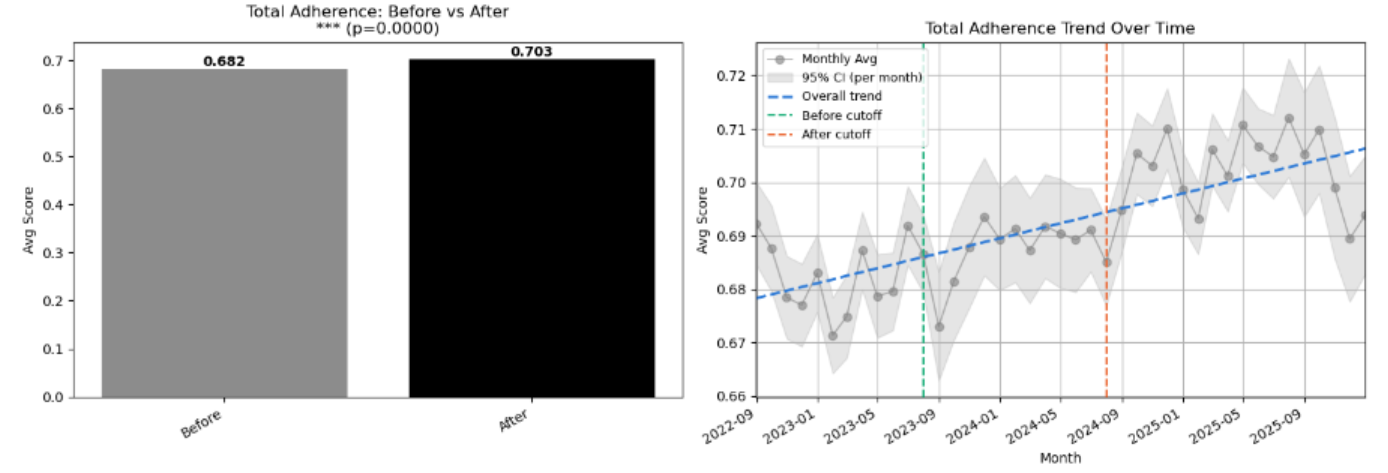
\includegraphics[width=\textwidth]{figures/adherence_trend.png}
    \caption{
    Changes in overall guideline adherence across the study period.
    \textbf{Left:} Mean overall adherence scores during the predefined
    pre-intervention (August 2022--July 2023) and post-intervention
    (August 2024--December 2025) periods.
    \textbf{Right:} Monthly mean overall adherence scores with 95\%
    confidence intervals across the study period. Vertical dotted lines
    delimit the transition/intervention period excluded from the primary
    pre--post comparison, and the dashed line indicates the overall
    temporal trend.
    }
    \label{fig:adherence-trend}
\end{figure}


\subsection{Guideline Adherence and Clinical Outcomes}

\subsubsection{Overall Adherence and 30-Day Mortality}

Higher adherence was associated with lower 30-day mortality
(Figure~\ref{fig:adherence-mortality}). Survivors had a higher mean
adherence score than those who died ($0.693$ vs.\ $0.652$, $p<0.001$), and
mortality fell across adherence strata, from 11\% at the bottom to roughly
3\% among admissions scoring $0.90$--$1.00$. On the continuous score, each
$0.1$-point increase carried $16.8\%$ lower odds of death (OR $=0.832$,
95\% CI $[0.811, 0.853]$), so the association is graded rather than
threshold-like. Adjusting for age, sex, comorbidity burden and hospital left
it intact (adjusted OR $=0.757$, 95\% CI $[0.727, 0.788]$, per
one-standard-deviation increase).

\begin{figure}[t]
    \centering
    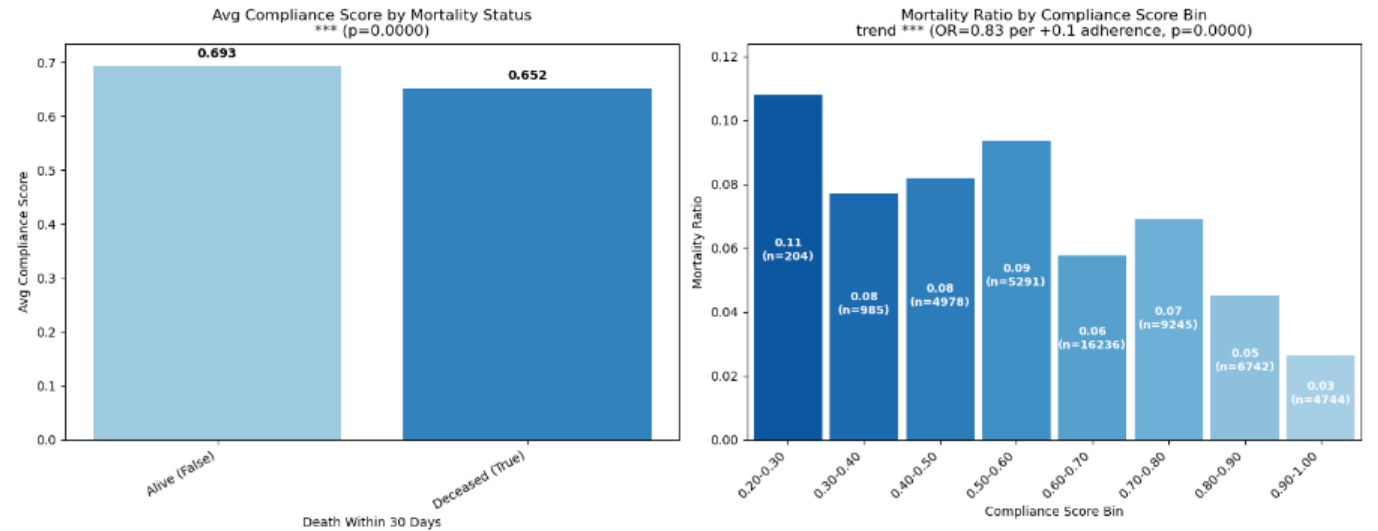
\includegraphics[width=\textwidth]{figures/adherence_mortality.png}
    \caption{
    Association between overall guideline adherence and 30-day mortality.
    \textbf{Left:} Mean overall adherence scores among patients who survived
    and those who died within 30 days.
    \textbf{Right:} Observed 30-day mortality rates across strata of overall
    adherence score; the number of admissions in each stratum is shown
    within the corresponding bar. Strata containing fewer than 30 admissions
    are not shown. The trend statistic reported above the panel is from
    logistic regression on the continuous adherence score, not on the
    binned values, and is expressed as the odds ratio per $0.1$-point
    increase in adherence.
    }
    \label{fig:adherence-mortality}
\end{figure}

\subsubsection{Insulin-Guideline Adherence and Hypoglycemia}

Adherence to the insulin-management recommendations showed negligible
correlation with subsequent hypoglycemic burden---measured as the proportion
of hospitalization days with events---for both hypoglycemia ($r=0.052$) and
severe hypoglycemia ($r=0.056$; $n=40{,}719$).

\subsection{Identifying Outcome-Associated Guideline Recommendations}

One model was fitted per complication per observation window, with adherence
and baseline covariates entered jointly (Table~\ref{tab:firth-summary}).
Between 9 and 34 predictors were retained per outcome, but the number
surviving all three window definitions ranged from none to 32, tracking
event frequency: mortality yielded the most robust predictors and the rarer
complications few or none. Mortality therefore serves as the worked example
below.

\begin{table}[t]
\centering
\caption{Summary of the bias-reduced (Firth) regression models.
Positive-event counts are shown for each observation-window definition.
Retained features denote predictors that remained significant after FDR
correction and pruning of highly correlated features. Robust features
remained statistically significant with the same effect direction across
all three observation-window definitions. MI, myocardial infarction;
AKI, acute kidney injury.}
\label{tab:firth-summary}

\begin{tabularx}{\textwidth}{
>{\raggedright\arraybackslash}X
ccccc
}
\toprule
Outcome & 24 h & 48 h & 72 h &
Retained & Robust \\
\midrule

Inpatient MI & 175 & 125 & 90 & 13 & 0 \\
30-day mortality & 3130 & 3130 & 2793 & 34 & 32 \\
Hyperglycemia & 8565 & 2153 & 1135 & 13 & 0 \\
Hyperosmolarity & 75 & 58 & 45 & 9 & 0 \\
Hypoglycemia & 2437 & 1742 & 1234 & 24 & 0 \\
Infection & 898 & 475 & 291 & 12 & 2 \\
Ketoacidosis & 46 & 33 & 25 & 9 & 0 \\
Inpatient AKI & 1362 & 901 & 655 & 21 & 5 \\
Severe hyperglycemia & 10019 & 4328 & 2376 & 28 & 8 \\
Severe hypoglycemia & 1686 & 1207 & 851 & 22 & 0 \\

\bottomrule
\end{tabularx}
\end{table}

\subsubsection{Component-Level Feature Importance}

Figure~\ref{fig:death-importance} shows the mortality profile. The model
recovered well-established clinical predictors---age, RDW, BMI, dementia,
cardiovascular comorbidity---which gives the approach face validity, and
several adherence components ranked among the strongest retained predictors:
routine basal insulin administration, routine glucose monitoring, insulin
following hyperglycemia, and admission creatinine assessment.

\begin{figure}[t]
    \centering
    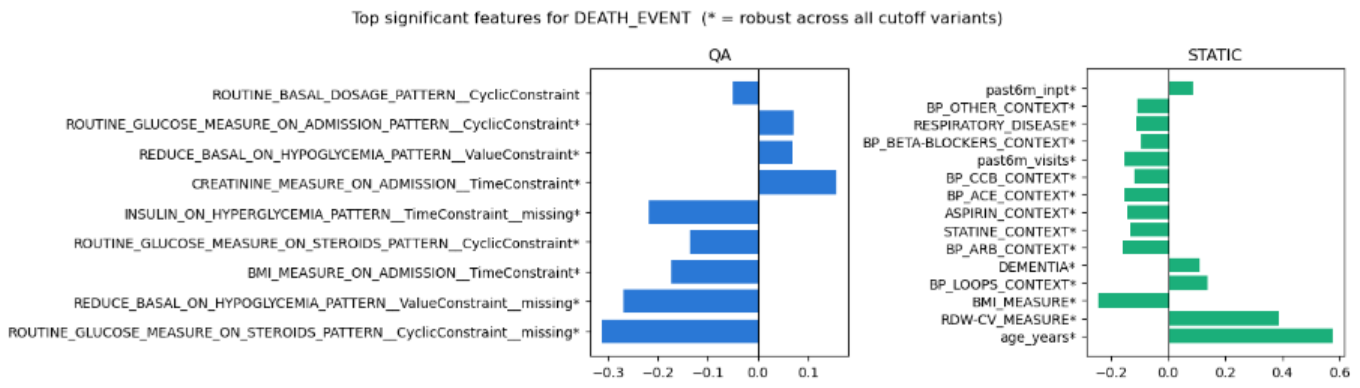
\includegraphics[width=\textwidth]{figures/death_feature_importance.png}
    \caption{
    Retained feature profile for 30-day mortality. The left panel shows
    retained guideline-adherence (QA) features and the right panel shows
    retained baseline clinical variables. Bar direction indicates the sign
    of the regression coefficient, while bar magnitude reflects the
    relative contribution after FDR correction and correlation pruning.
    Features marked with an asterisk persisted across all three
    observation-window definitions.
    }
    \label{fig:death-importance}
\end{figure}

\subsubsection{Recurring Guideline Recommendations Across Clinical Outcomes}

Synthesizing the adherence features across all outcome models
(Figure~\ref{fig:recurring-guidelines}), insulin following hyperglycemia and
admission glucose monitoring recurred most broadly, followed by BMI and
creatinine assessment on admission and monitoring during corticosteroid
treatment; basal-dose components appeared in fewer, more outcome-specific
models. Direction was not uniform---the same component could carry opposite
signs for different endpoints.

\begin{figure}[t]
    \centering
    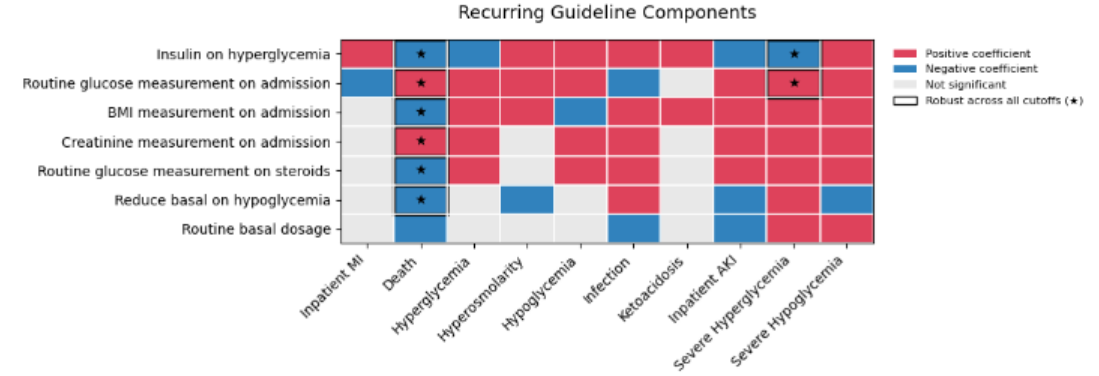
\includegraphics[width=\textwidth]{figures/recurring_guideline_components.png}
    \caption{
    Recurring guideline-adherence components identified by the bias-reduced
    regression models across clinical outcomes. Rows correspond to guideline
    recommendations and columns to clinical outcomes. Colored cells indicate
    statistically significant associations after FDR correction
    (red: positive regression coefficient; blue: negative regression
    coefficient). Stars denote associations that remained significant with
    a consistent direction across all three observation-window definitions
    (24, 48, and 72 hours). Blank cells indicate no statistically significant
    association.
    }
    \label{fig:recurring-guidelines}
\end{figure}

\subsection{Propensity-Weighted Evaluation of Guideline Adherence}

Because these models quantify conditional predictive associations rather
than treatment effects, both overall adherence and the recurrent components
were re-evaluated using inverse probability of treatment weighting (IPTW),
contrasting admissions above the median adherence score with those at or
below it. The overall-adherence analyses achieved satisfactory covariate
balance (maximum post-weighting standardized mean difference $<0.08$).

\subsubsection{Overall Guideline Adherence}

Relative to the low-adherence group, above-median adherence carried 44\%
lower odds of 30-day mortality (OR $=0.557$, 95\% CI $[0.514, 0.603]$),
82\% lower odds of hyperglycemia (OR $=0.175$, 95\% CI $[0.154, 0.199]$) and
52\% lower odds of severe hyperglycemia (OR $=0.485$, 95\% CI
$[0.450, 0.523]$), all FDR-adjusted $p<0.001$, against 20\% higher odds of
hypoglycemia (OR $=1.204$, 95\% CI $[1.090, 1.331]$, $p<0.001$;
Table~\ref{tab:iptw-overall}). Nothing survived correction for inpatient
myocardial infarction (MI), hyperosmolarity, infection, ketoacidosis or
inpatient acute kidney injury (AKI).

The asymmetry between those two directions is the substantive result: the
reduction in hyperglycemic burden is roughly ninefold larger on the log-odds
scale than the accompanying increase in hypoglycemia, and the increase in
\emph{severe} hypoglycemia did not reach significance (OR $=1.129$,
$p_{\mathrm{FDR}}=0.096$).

\subsubsection{Individual Guideline Recommendations}

We next examined the recurrent guideline recommendations identified above
using separate IPTW models (Table~\ref{tab:iptw-patterns}).
Only a subset of the recurrent predictors remained significant after
propensity weighting, indicating that several predictive associations were
largely explained by differences in baseline patient characteristics.

Of the significant associations, a further six were set aside because
propensity weighting failed to achieve acceptable covariate balance
(maximum post-weighting SMD between $0.90$ and $2.46$, against a
prespecified threshold of $0.10$). All six concerned BMI or creatinine
measurement on admission, for which adherence is near-universal
(mean $0.87$ and $0.98$ respectively, both with median $1.00$), so that
dichotomizing at the median produces groups too dissimilar to balance. The
corresponding coefficients were numerically degenerate and are not
interpretable; these component--outcome pairs are therefore reported as
non-estimable rather than as findings.

Eight associations were both significant and adequately balanced.
Above-median adherence to routine basal insulin dosing (OR $=0.748$),
routine glucose monitoring (OR $=0.870$) and insulin administration
following hyperglycemia (OR $=0.907$) each remained associated with lower
30-day mortality. For glycemic outcomes, insulin following hyperglycemia
(OR $=0.220$, 78.0\% lower odds) and routine basal insulin dosing
(OR $=0.402$, 59.8\% lower odds) were associated with substantially lower
odds of subsequent severe hyperglycemia, while insulin following
hyperglycemia also carried 28.3\% higher odds of hypoglycemia
(OR $=1.283$)---the same trade-off seen at the level of overall adherence.

These are the same components that showed the largest implementation gaps.
Insulin following hyperglycemia (mean adherence $0.15$) and routine basal
insulin dosing ($0.21$--$0.23$) are simultaneously the least-implemented
recommendations assessed and, after weighting, among those most strongly
associated with mortality and with severe hyperglycemia.

Adherence to glucose monitoring on admission was associated with a higher
recorded incidence of hyperglycemia (OR $=2.664$) and severe hyperglycemia
(OR $=2.121$). Since these outcomes are ascertained from glucose
measurements, more frequent early measurement mechanically increases the
chance of recording an event, so both associations likely reflect
ascertainment rather than harm. This component was retained, unlike routine
monitoring throughout the admission, which was excluded from the glycemic
models because it overlaps the detection window directly rather than being
bounded to the first days.

\begin{table}[t]
\centering
\caption{Inverse probability of treatment weighting (IPTW) analysis of
overall guideline adherence. Adherence was dichotomized at the median of
each outcome's eligible population; coefficients from the weighted logistic
regression models are therefore log-odds ratios comparing the above-median
with the at-or-below-median adherence group, and OR $=\exp(\beta)$ is the
corresponding odds ratio. Confidence intervals are unadjusted; $p$-values
were adjusted across outcomes using the Benjamini--Hochberg false discovery
rate (FDR) procedure. Covariate balance was assessed using the maximum
standardized mean difference (SMD) after weighting. MI, myocardial
infarction; AKI, acute kidney injury.}
\label{tab:iptw-overall}

\small
\setlength{\tabcolsep}{4pt}

\begin{tabular}{lrrrrr}
\toprule
Outcome & $\beta$ & OR & 95\% CI (OR) & Max SMD & $p_{\mathrm{FDR}}$ \\
\midrule
Hyperglycemia
    & $-1.742$ & 0.175 & [0.154, 0.199] & 0.019 & $<0.001$ \\

Severe hyperglycemia
    & $-0.724$ & 0.485 & [0.450, 0.523] & 0.012 & $<0.001$ \\

30-day mortality
    & $-0.586$ & 0.557 & [0.514, 0.603] & 0.020 & $<0.001$ \\

Hypoglycemia
    & $0.186$ & 1.204 & [1.090, 1.331] & 0.034 & $<0.001$ \\

Severe hypoglycemia
    & $0.121$ & 1.129 & [1.001, 1.274] & 0.030 & 0.096 \\

Hyperosmolarity
    & $0.106$ & 1.112 & [0.652, 1.896] & 0.020 & 0.800 \\

Ketoacidosis
    & $0.116$ & 1.123 & [0.561, 2.246] & 0.021 & 0.800 \\

Inpatient MI
    & $0.055$ & 1.057 & [0.732, 1.523] & 0.020 & 0.800 \\

Infection
    & $-0.025$ & 0.975 & [0.809, 1.175] & 0.020 & 0.800 \\

Inpatient AKI
    & $0.018$ & 1.018 & [0.888, 1.168] & 0.022 & 0.800 \\

\bottomrule
\end{tabular}
\end{table}

\begin{table}[t]
\centering
\caption{Inverse probability of treatment weighting (IPTW) analysis of
individual guideline recommendations. Rows are the component--outcome pairs
that were both statistically significant after FDR correction and adequately
balanced after weighting (maximum standardized mean difference
$<0.10$). Adherence to each recommendation was dichotomized at the median of
its eligible population, so coefficients compare above-median with
at-or-below-median adherence and OR $=\exp(\beta)$. Confidence intervals are
unadjusted; $p$-values were adjusted using the Benjamini--Hochberg false
discovery rate (FDR) procedure. A further six significant associations, all
concerning BMI or creatinine measurement on admission, failed the balance
criterion (maximum SMD $0.90$--$2.46$) and are not reported.
$^{\dagger}$Likely to reflect ascertainment rather than harm: the outcome is
detected from glucose measurements, so more frequent early measurement
increases the opportunity to record an event.}
\label{tab:iptw-patterns}

\small
\setlength{\tabcolsep}{4pt}

\begin{tabular}{llrrrr}
\toprule
Outcome & Recommendation & $\beta$ & OR & 95\% CI (OR) & $p_{\mathrm{FDR}}$ \\
\midrule

30-day mortality & Routine basal dosage
    & $-0.291$ & 0.748 & [0.691, 0.809] & $<0.001$ \\

30-day mortality & Routine glucose monitoring
    & $-0.139$ & 0.870 & [0.809, 0.937] & $<0.001$ \\

30-day mortality & Insulin after hyperglycemia
    & $-0.098$ & 0.907 & [0.842, 0.977] & 0.011 \\

\midrule

Severe hyperglycemia & Insulin after hyperglycemia
    & $-1.514$ & 0.220 & [0.202, 0.239] & $<0.001$ \\

Severe hyperglycemia & Routine basal dosage
    & $-0.912$ & 0.402 & [0.372, 0.434] & $<0.001$ \\

Severe hyperglycemia & Admission glucose monitoring$^{\dagger}$
    & $0.752$ & 2.121 & [1.974, 2.280] & $<0.001$ \\

\midrule

Hyperglycemia & Admission glucose monitoring$^{\dagger}$
    & $0.980$ & 2.664 & [2.389, 2.971] & $<0.001$ \\

\midrule

Hypoglycemia & Insulin after hyperglycemia
    & $0.249$ & 1.283 & [1.163, 1.416] & $<0.001$ \\

\bottomrule
\end{tabular}
\end{table}


% discussion.tex already begins with \section{Discussion}
\section{Discussion}
\label{sec:discussion}

\subsection{Principal Findings}

Taken together, these analyses show that implementation of the national
recommendations for hyperglycemia treatment in hospitalized patients was
associated with improved adherence across multiple guideline
recommendations. Higher overall adherence was consistently associated with
lower mortality and reduced hyperglycemic complications, while the
component-level regression and propensity-weighted analyses identified
routine glucose monitoring, basal insulin management, and insulin treatment
of hyperglycemia as the guideline components most consistently associated
with subsequent clinical outcomes.

Adherence was not uniform across the assessed recommendations. Near-universal
implementation was observed for several admission and medication-management
recommendations, whereas the largest gaps were concentrated in insulin
management---administration of insulin following hyperglycemia, routine
basal insulin dosing, and bolus dose reduction following hypoglycemia. This
pattern separates recommendations that can be satisfied by a single
discrete action, such as ordering a laboratory test or discontinuing a
medication on admission, from those requiring repeated insulin decisions
across the hospitalization.

The improvement following implementation was significant but modest, and the
$p$-value reflects the number of admissions rather than the size of the
effect. It was also accompanied by substantial inter-hospital heterogeneity,
with center-level trajectories ranging from improvement through no change to
modest decreases; the data do not identify what drove that divergence.

In the component-level models, adherence features ranked among the strongest
retained predictors alongside established clinical variables such as age,
RDW, BMI and dementia---the practical requirement for treating them as
monitorable quality targets rather than retrospective descriptors.

The clearest outcome signal was for 30-day mortality. In the
propensity-weighted analysis, which scores adherence over a fixed
early-admission window and so preserves temporal precedence of exposure over
outcome, above-median adherence carried 44\% lower odds of death
(OR $=0.557$, 95\% CI $[0.514, 0.603]$). Two descriptive estimates agree in
direction: whole-admission adherence adjusted for age, sex, comorbidity and
hospital (OR $=0.757$ per SD), and a graded fall across the adherence range
rather than only between groups (OR $=0.832$ per $0.1$ point). A graded
association is harder to explain by a simple high-versus-low difference in
case mix, though it shares the whole-admission timing concern discussed
below. Because the three use different exposure definitions and windows they
corroborate direction, not magnitude; the propensity-weighted estimate is
primary, being the only one whose exposure window is guaranteed to precede
the outcome.

The glycemic findings show a favorable risk profile. Above-median adherence
was associated with substantially lower odds of hyperglycemia (OR $=0.175$)
and severe hyperglycemia (OR $=0.485$), while the accompanying rise in
hypoglycemia was small (OR $=1.204$) and the association with \emph{severe}
hypoglycemia did not survive correction (OR $=1.129$, $p=0.096$). The same
asymmetry appears in the unadjusted insulin-adherence correlations
($r=0.052$ and $r=0.056$) and at component level, where insulin following
hyperglycemia tracked lower severe hyperglycemia alongside more
hypoglycemia. Greater adherence therefore bought a large reduction in
hyperglycemic burden at the cost of a small increase in mild hypoglycemia
and no detectable increase in severe hypoglycemia---the balance the
recommendations are intended to strike. Since non-significance is not
evidence of absence, the severe-hypoglycemia result shows no signal of harm
at this sample size rather than establishing that none exists.

These findings have no direct precedent against which to be compared. The
position paper assessed here was issued in 2023, and no prior study has
measured adherence to it, at this scale, or across a national
implementation; the methods used to derive the adherence measure are
likewise applied here for the first time in this setting
(Section~\ref{sec:related-work}). The results are therefore reported as a
first characterization of how the recommendations were adopted and of which
of them track subsequent outcomes, rather than as a replication or
contradiction of earlier estimates.

\subsection{Strengths and Limitations}

The principal strengths of this work are the scale and breadth of the
cohort---48,354 admissions across six general hospitals---and the automated,
component-level assessment of guideline adherence, which permits each
recommendation to be evaluated separately rather than as an aggregate
compliance score. Analyses were repeated across three observation-window
definitions, and only associations that persisted with a consistent effect
direction across all three were treated as robust. In the component-level
and propensity-weighted models, adherence was scored only over the first
24, 48, or 72 hours of admission, while complications occurring before the
corresponding cutoff were excluded; because admissions were at least 48
hours long by inclusion, exposure therefore strictly precedes outcome in
these analyses. The adherence--outcome associations were additionally
approached in two complementary ways: regression adjustment, which
accommodates adherence as a continuous score and yields a conditional
estimate, and propensity weighting, which contrasts balanced high- and
low-adherence groups and yields a marginal estimate whose covariate balance
can be verified directly. Agreement in direction between two designs with
different assumptions is more informative than either alone.

Several limitations qualify these findings. The design is observational, and
none of the estimates should be read as causal effects. Residual confounding
remains throughout: weighting balances only measured covariates, and
unmeasured factors---real-time illness severity above all, and decisions to
limit or de-escalate treatment---cannot be excluded. The component-level
models quantify conditional predictive associations, and direction was not
uniform across outcomes: the same component could carry opposite signs for
different endpoints, reflecting differences in clinical context, indication
and applicability.

The mortality analyses divide by exposure definition. The component-level
and propensity-weighted models score adherence over a fixed early-admission
window, so exposure strictly precedes outcome and reverse causation is not a
concern. The adjusted estimate (OR $=0.757$) instead averages adherence over
the whole admission and is descriptive: because 30-day mortality is
predominantly an end-of-admission event, and guideline-concordant management
is frequently de-escalated in patients on a deteriorating trajectory, that
average incorporates the period immediately preceding death, where adherence
may reflect the course of care rather than determine it.

Dichotomizing adherence at the median, as the weighting requires, discards
dose-response information and costs power; because the threshold is
population-relative it also does not correspond to a fixed adherence value
across outcomes. Generalized propensity-score methods would permit a
balance-verified dose-response estimate at the cost of modelling the
exposure distribution; for now dose-response is characterized only
descriptively, by the continuous-score trend.

Adherence and outcomes were ascertained during the same hospitalization, and
detecting glycemic events depends on glucose being measured. Routine glucose
monitoring was therefore excluded from the glycemic models, though residual
detection effects may remain for other monitoring recommendations. The
pre--post comparison is also uncontrolled, so secular trends in inpatient
care cannot be separated from the implementation itself. The non-mortality
models do not account for the competing risk of death, which biases those
endpoints conservatively. And the findings come from adult inpatients in
Israeli general hospitals under a single national guideline, so both the
adherence levels observed and the components that proved most consequential
may differ in other health systems or under different recommendations.
Finally, the data is assembled from hospital admissions rather than from a
longitudinal record, so chronic diagnoses managed in the community may be
incompletely captured---a patient whose diabetes is followed in primary care
may arrive with no diabetes diagnosis coded. Ascertaining eligibility and the
glycemic outcomes from glucose measurements rather than diagnosis codes
limits the consequences, but the comorbidity score and the reported
proportion of hyperglycemic admissions carrying a documented diagnosis are
both likely to be understated. Cross-site coding heterogeneity, by contrast,
was not a material concern, since the records were harmonized to a common
coding system as part of the Kineret project.

\subsection{Implications}

The most actionable pattern in these results is a convergence. The
recommendations showing the largest implementation gaps---administration of
insulin following hyperglycemia, and the frequency and dose components of
routine basal insulin---are also among those most consistently associated
with subsequent outcomes after balancing measured baseline characteristics.
The components where practice departs most from the guideline are therefore
not peripheral ones, and this convergence identifies them as natural targets
for decision support: they are repeated insulin decisions distributed
across a hospitalization, which is precisely the kind of task where a
prompt at the point of care can plausibly help, and unlike the
single-action admission recommendations they are not already at ceiling.

This should not be read as an attribution of fault. A low adherence score
records that the action expected by the guideline is absent from the record,
not that the decision was wrong. Ward-level judgment---a patient not eating,
an imminent procedure, a deliberate decision to tolerate higher glucose in a
frail patient---is frequently the correct reason for a departure, and none
of it is recoverable from records collected for clinical rather than
research purposes. The measure is a population-level statistic, not an
assessment of individual clinicians or centers, and the inter-hospital
variation reported here should be read in the same way.

The work is accordingly a retrospective characterization, not a
decision-support system: it issues no recommendations, returns nothing to
the treating team, and no prospective deployment is currently planned. What
it offers is a measurement instrument---an automated, component-level and
transferable way to ask whether a guideline was followed and which of its
recommendations track outcomes, a question that has until now required chart
review and cannot be answered at national scale by that means.

\subsection{Future Work}

Nothing restricts the approach to recommendations a guideline already
contains. Because each is declared externally as a pattern rather than
implemented in analysis code, candidate patterns cost no more to add than
existing ones: a practice merely suspected to matter, or a variant of a
current recommendation with a different threshold or window, can be encoded
and evaluated by exactly the procedure used here. The instrument is
indifferent to whether the pattern it scores is a rule anyone has yet
endorsed.

That inverts the question. Rather than asking only whether an existing
guideline was followed, one could ask which candidate practices earn a place
in it, and---more uncomfortably---which current recommendations do not track
outcomes at all. Guideline development is presently a consensus exercise
informed by trial evidence that is expensive to generate and often
unavailable for the operational details a guideline must nonetheless fix,
such as how many hours after a hyperglycemic reading correction insulin
should follow. Screening candidate patterns against routinely collected
records offers a cheap way to prioritize which of those details are worth
resolving properly.

Two cautions apply. Such associations would be observational, and
confounding by indication is strongest exactly where a practice is applied
selectively, so candidates surfaced this way would be hypotheses for
prospective evaluation rather than conclusions. And multiplicity grows with
the candidate space, so a search over many hypothesized patterns would need
correction considerably more conservative than that applied here.


% conclusion.tex already begins with \section{Conclusion}
\section{Conclusion}
\label{sec:conclusion}

Adherence to a national inpatient hyperglycemia guideline can be measured
automatically, at the level of its individual recommendations, across an
entire hospital network. Applying that measurement to 48,354 admissions in
six Israeli general hospitals shows that adherence improved after the
guideline was issued, that the improvement was modest and unevenly
distributed across both recommendations and centers, and that adherence is
associated with lower 30-day mortality and a lower burden of hyperglycemic
complications once measured baseline differences are balanced.

The recommendations that were least well implemented are largely the same
ones whose adherence tracks subsequent outcomes: the repeated insulin
decisions distributed across a hospitalization, rather than the
single discrete actions taken on admission. That convergence, together with
the favorable shift in glycemic risk---substantially less hyperglycemia at
the cost of slightly more mild hypoglycemia and no detectable increase in
severe hypoglycemia---is the evidence a guideline needs in order to justify
the effort of implementing it more completely.

These are associations rather than treatment effects, and they describe how
a guideline was adopted rather than how well any clinician practised. What
the work establishes is that the question is now answerable at scale: which
recommendations within a guideline are followed, and which of them make a
difference, can be asked of an entire health system's records rather than of
a sample small enough to review by hand.


% --------------------------------------------------
% End matter
% --------------------------------------------------
\section*{CRediT Authorship Contribution Statement}
\textbf{Shahar Oded:} Conceptualization, Methodology, Software, Validation,
Formal analysis, Data curation, Visualization, Writing -- original draft.
\textbf{Yuval Shahar:} Conceptualization, Methodology, Supervision, Funding
acquisition, Writing -- review \& editing.
\textbf{Erez Shalom:} Resources, Project administration, Writing -- review \&
editing.
\textbf{Amir Bashkin:} Investigation, Resources, Writing -- review \& editing.
\textbf{Leonard Saiegh:} Investigation, Resources, Writing -- review \& editing.
\textbf{Dror Cantrell:} Investigation, Resources, Writing -- review \& editing.
\textbf{Irit Wirsansky:} Investigation, Resources, Writing -- review \& editing.
\textbf{Muhamad Badarne:} Investigation, Resources, Writing -- review \& editing.
\textbf{Irena Barash:} Investigation, Resources, Writing -- review \& editing.
\textbf{Avivit Cahn:} Conceptualization, Investigation, Writing -- review \&
editing.
\textbf{Irit Hochberg:} Conceptualization, Methodology, Validation,
Resources, Supervision, Writing -- review \& editing.

\section*{Funding}
This research was funded by the Israeli Ministry of Science and Technology
Kineret Grant No.~0006850 (Governmental Project No.~1001701806), the Israeli
National Health Policy Grant No.~2020/284, the Israel Precision Medicine
Partnership (IPMP) Grant No.~3543/21, and the European Union's Horizon Europe
research and innovation programme under Grant Agreement No.~101156210
[CARAMEL]. The funders had no role in study design, data collection and
analysis, decision to publish, or preparation of the manuscript.

\section*{Declaration of Competing Interest}
Several of the authors contributed to the national position paper whose
implementation is assessed in this study. The authors declare no competing
financial interests or personal relationships that could have appeared to
influence the work reported in this paper.

\section*{Data Availability}
The abstraction engine, the knowledge base of temporal-abstraction and
quality-assessment definitions, and the analysis notebooks are publicly
available in the Mediator repository \citep{mediator-github}, and the
extraction and cohort-construction pipeline in a companion repository
\citep{kineret-etl-github}. The curated concept indices mapping the source
vocabulary onto the concepts named in the knowledge base are provided as
supplementary material.

All processing and analysis were performed inside a closed hospital
computing environment. The code released here is a replica of that
pipeline; no source data, intermediate datasets, or unaggregated outputs
leave that environment, and the results reported in this paper are exported
aggregate statistics. The underlying patient-level electronic health record
data cannot be shared, as it comprises identifiable clinical records
governed by the approvals under which it was obtained.

\section*{Ethics Approval}
The study was approved by the institutional Helsinki committee of each
participating center under a common protocol (NHR-0152-23): Galilee Medical
Center (NHR-0152-23), Hillel Yaffe Medical Center (HYMC-0074-24), Shamir
Medical Center (ASF-0117-24), Tzafon Medical Center (POR-0047-24), Barzilai
University Medical Center (BRZ-0059-24), and Bnai Zion Medical Center
(BNZ-0067-24). Recruitment was approved for up to 30,000 participants across
all centers combined. A full waiver of informed consent was granted, since
the study extracts records from a de-identified repository with no patient
contact.

\section*{Acknowledgements}
This study would not have been possible without the Kineret project team,
who built and maintain the harmonized multicenter data warehouse on which it
rests. Transforming the records of a national hospital network into a
common data model, and sustaining the infrastructure and governance that
make it usable for research, represents a substantial body of work in its
own right; the authors are grateful for that effort and for the team's
support in accessing the data and extracting the study cohort. The authors
also thank the Helsinki committee coordinators at the participating centers
for their assistance throughout the approval process.

\bibliographystyle{elsarticle-num}
\bibliography{references}

% appendix.tex begins with \appendix
\appendix

\section{Data Preparation Details}
\label{app:data-prep}

\paragraph{Source and unified tables.}
The extraction consumed the OMOP tables \texttt{person},
\texttt{visit\_occurrence}, \texttt{visit\_detail}, \texttt{death},
\texttt{condition\_occurrence}, \texttt{observation},
\texttt{procedure\_occurrence}, \texttt{device\_exposure},
\texttt{drug\_exposure}, and \texttt{measurement}, and reorganized them into
five unified tables: \emph{visits}, \emph{visit types}, \emph{clinical
events} (conditions, observations, procedures, and device exposures under a
common schema), \emph{drug exposures}, and \emph{measurements}. The only
enrichments applied were the attachment of Anatomical Therapeutic Chemical
(ATC) codes to drug exposures, where available, the harmonization of column
types, and the closing of intervals whose end timestamp was missing or not
later than their start one second after their start, so that point
observations stored under an interval schema carry an explicit rather than a
degenerate duration. Dimension tables enumerating the distinct clinical,
measurement, and drug concepts, together with their units and administration
routes, were derived from the unified tables and used to support concept
curation.

\paragraph{Concept curation.}
Candidate codes for each target concept were surfaced by descriptive
analytics over the dimension tables, ranked by frequency of occurrence and
by apparent relevance to the concept, and then accepted or rejected by the
clinical domain expert. The resulting indices define both the concepts
included in the abstraction input and the departmental and diagnostic
exclusions applied in the cohort definition.

\paragraph{Derived concepts.}
Body mass index was computed from paired height and weight measurements
where not recorded directly. Ketoacidosis events were derived from
combinations of pH, bicarbonate, and intravenous insulin administration, as
described in Appendix~\ref{app:definitions}.

\paragraph{Modified Charlson comorbidity index.}
The score is a weighted sum of ten chronic condition flags ascertained from
the first 48 hours of admission: malignancy, chronic kidney disease, and
chronic liver disease weighted 2; and cardiac disease, chronic respiratory
disease, diabetes, dementia, alcohol misuse, anemia, and recurrent falls
weighted 1. One additional point is added per decade of age above 50.
Categories absent from the original Charlson instrument reflect the
condition groupings that could be resolved from the unmapped source
vocabulary during curation.

\section{Operational Definitions of Complications}
\label{app:definitions}

Definitions are given in the order used in the Results tables. As described
in Section~\ref{sec:methods}, the glycemic endpoints and acute kidney injury
are derived within the knowledge base from the corresponding measurements,
while ketoacidosis, infection, hyperosmolality and myocardial infarction were
computed during data preparation and supplied to the engine as primitive
concepts.

\paragraph{Thirty-day mortality.}
Death recorded in the linked mortality data between 14 days before and 30
days after the recorded discharge datetime. The backward tolerance ensures
that in-hospital deaths are captured where the death record precedes the
administrative discharge timestamp.

\paragraph{Hyperglycemia.}
Either a single glucose measurement $\geq250$ mg/dL, or a sustained
hyperglycemic state, defined as a glucose measurement $\geq180$ mg/dL whose
immediately preceding measurement within the previous 24 hours was also
$\geq180$ mg/dL. The sustained-state requirement prevents an isolated
elevated reading from being counted as a complication.

\paragraph{Severe hyperglycemia.}
Any single glucose measurement $\geq250$ mg/dL. This endpoint overlaps by
construction with hyperglycemia and is retained as a separate, more specific
target.

\paragraph{Hypoglycemia.}
Either a single glucose measurement $\leq54$ mg/dL, or a sustained
hypoglycemic state, defined as a glucose measurement $\leq70$ mg/dL whose
immediately preceding measurement within the previous 24 hours was also
$\leq70$ mg/dL.

\paragraph{Severe hypoglycemia.}
Any single glucose measurement $\leq54$ mg/dL.

\paragraph{Inpatient acute kidney injury (AKI).}
Laboratory-defined AKI of stage 2 or above, established either by a serum
creatinine ratio $\geq2.0$ relative to the patient's baseline, or by an
absolute serum creatinine $\geq4.0$ mg/dL. Stage~1 injury was deliberately
excluded from the endpoint.

\paragraph{Inpatient myocardial infarction (MI).}
Evidence of an ischemic cardiac event---ischemic heart disease, myocardial
infarction, coronary intervention, cardiac catheterization, or
revascularization---together with a troponin measurement of at least 600.
The troponin requirement excludes coded cardiac history unaccompanied by
biochemical evidence of acute injury.

\paragraph{Hyperosmolality.}
Emitted by either of two paths. The derived path implements a
hyperosmolar-hyperglycemic-state rule: for each glucose measurement
$\geq600$ mg/dL, the nearest serum sodium measurement within $\pm6$ hours is
located and the effective osmolality computed as
$2 \times \mathrm{Na} + \mathrm{glucose}/18$; an event is emitted where this
exceeds 320 mOsm/kg, provided no acidosis event occurs within $\pm6$ hours
of the triggering glucose draw. The acidosis exclusion separates
hyperosmolar states from diabetic ketoacidosis. The observation path
additionally emits an event wherever hyperosmolality is directly coded.

\paragraph{Ketoacidosis.}
Emitted by either of two paths. The observation path emits an event wherever
ketoacidosis is directly coded. The derived path requires the conjunction of
a pH measurement $\leq7.3$, a bicarbonate measurement $\leq10$ mEq/L within
24 hours of it, and intravenous insulin administration within 6 hours of
it---that is, biochemical acidosis together with the treatment response it
implies.

\paragraph{Infection.}
Requires a physiological trigger, corroborating diagnostic evidence, and
treatment, all within a single episode. The trigger is any one of: fever
onset, defined as at least two body-temperature measurements $\geq37.8^\circ$C
where all temperatures in the preceding 48 hours were $\leq37.7^\circ$C;
leukocytosis, defined as a white-cell count $\geq11$ where counts in the
preceding 48 hours lay between 4 and 11; leukopenia, defined as a white-cell
count $\leq4$ under the same prior-stability condition; or neutropenia,
defined as a neutrophil count $\leq1.5$ where preceding counts within 48
hours exceeded 1.5. Diagnostic evidence requires at least one blood culture,
urine culture, or chest radiograph within $\pm24$ hours of the trigger, the
latest such record within the window serving as the episode anchor.
Treatment requires at least one antibiotic administration after that anchor
and within 72 hours of the trigger. Triggers occurring within 72 hours of an
already-accepted event are collapsed into it, so an admission may contribute
multiple distinct episodes. The prior-stability condition attached to every
trigger restricts the endpoint to infections arising during the
hospitalization rather than present on admission.

\section{Assessed Guideline Recommendations}
\label{app:patterns}

Fourteen quality-assessment patterns were evaluated, corresponding to the
components reported in the Results
(Table~\ref{tab:pattern-definitions}). Each pattern defines an applicability
condition, so that it is scored only for admissions and time points at which
the underlying recommendation applies, and one or more compliance aspects.
Three aspect types are used: \emph{time}, whether a required action occurred
within a required interval; \emph{cyclic}, whether a recurring action
occurred at the required frequency; and \emph{value}, whether an
administered dose met the required magnitude. Insulin administration after
hyperglycemia is a limiting case of the time aspect: it is defined by an
overlap relation rather than by a delay, so no distance separates anchor
from action for a membership function to grade, and the constraint is
satisfied on existence alone---scoring 1 where the action is present and 0
where it is not.

\begin{table}[t]
\centering
\caption{Assessed guideline recommendations and their operational
definitions in the knowledge base.}
\label{tab:pattern-definitions}
\small
\begin{tabularx}{\textwidth}{
>{\raggedright\arraybackslash}p{0.30\textwidth}
l
>{\raggedright\arraybackslash}X
}
\toprule
Recommendation & Aspect & Operational definition \\
\midrule

Admission glucose monitoring & Cyclic &
Glucose measured in each 24-hour window over the first days of admission:
three days where diabetes is documented, two otherwise. Full credit at
three or more measurements per window, decaying linearly to zero at
none. \\

Routine glucose monitoring & Cyclic &
Glucose measured in each 24-hour window throughout the admission (evaluated
to 14 days). While glucose is in a hyperglycemic or hypoglycemic state, full
credit is given at three or more measurements per window. Under routine
conditions the trapezoid peaks at at least one measurement per window. \\

Glucose monitoring during corticosteroid therapy & Cyclic &
Glucose measured in each 24-hour window over the first two days of
corticosteroid treatment, with full credit at at least three measurements
per window. \\

BMI measurement on admission & Time &
Body mass index or weight recorded within 48 hours of admission, decaying
linearly to zero at 72 hours; a measurement recorded up to six months
before admission is carried forward as relevant. \\

Creatinine measurement on admission & Time &
Serum creatinine measured within 48 hours of admission, decaying linearly
to zero at 72 hours. Unlike BMI, no pre-admission measurement is carried
forward, so the measurement must fall within the admission itself. \\

Antidiabetic discontinuation on admission & Time &
Prescribed antidiabetic agents carrying high hypoglycemia risk discontinued
during the first 72 hours of admission, with credit decreasing linearly to
zero if an agent was administered during that time. \\

SGLT2 discontinuation on admission & Time &
Prescribed SGLT2 inhibitors discontinued during admission. Any in-hospital
administration scores 0, and the absence of one scores 1, assuming the
patient was treated with the agent at home. \\

Basal insulin continuation on admission & Time &
Basal insulin administered within 36 hours of admission for patients
established on basal insulin at home, decaying linearly to zero at 48
hours. \\

Insulin administration after hyperglycemia & Time &
Any dose of reactive bolus or intravenous insulin administered overlapping a
meal (2-hour window before or after the meal) while glucose is elevated. \\

Antidiabetic discontinuation after hypoglycemia & Time &
Prescribed antidiabetic agents withheld following a hypoglycemic event,
with credit increasing over 72 hours and full credit sustained
thereafter. \\

Basal dose reduction after hypoglycemia & Value &
Basal insulin dose reduced relative to the preceding dose following a
hypoglycemic event, scored on the ratio of the new dose to the preceding
one: any reduction receives full credit, declining to zero at an unchanged
dose. Unlike the bolus pattern below, hypoglycemic events \emph{not}
followed by a basal dose within 24 hours are scored as compliant rather than
excluded, following the convention that a withheld action satisfies the
recommendation. \\

Bolus dose reduction after hypoglycemia & Value &
Bolus insulin dose reduced following a hypoglycemic event, on the same dose
ratio and membership function as the basal pattern above, but evaluated only
where bolus insulin was actually administered within 24 hours of the event;
events with no subsequent bolus are excluded from scoring rather than
counted as compliant (assuming basal is routine and bolus is a reaction to
an event). \\

Routine basal dosage (frequency) & Cyclic &
Basal insulin administered in each 24-hour window through the first 14 days
of admission, evaluated in windows where hyperglycemia is present, with full
credit between one and four administrations per window and declining credit
beyond that range. \\

Routine basal dosage (dose) & Value &
Judged against body weight for patients not established on basal insulin at
home: full credit between 0.2 and 0.6 units per kilogram, rising from zero
below 0.2 and declining to zero at 1.0 units per kilogram, using a default
weight of 81~kg where no weight measurement is available. For patients
already receiving basal insulin at home, the established dose is accepted as
given and is not weight-normalized, assuming medical staff reacted to this
dose and might have increased the hospital dose due to tolerance. \\

\bottomrule
\end{tabularx}
\end{table}
Each aspect is scored by a trapezoidal membership function as described in
Section~\ref{sec:methods}, so the reported values are continuous on $[0,1]$:
full credit is given throughout the interval in which the recommendation is
considered met, with linear partial credit on either side of it and zero
beyond the outer bounds. Several trapezoids are deliberately open on one
side---full credit at or above a required count, for instance, with no
penalty for exceeding it---so that partial credit applies only where
departing from the recommendation in that direction is meaningful. A
recommendation carrying more than one aspect is reported under each aspect
separately, which is why routine basal dosage appears twice above---once for
the frequency of administration and once for the dose administered.

The differing treatment of unanswered anchors in the two dose-reduction
patterns is deliberate and reflects how the two insulins are used. Basal
insulin is given routinely, so a hypoglycemic event with no basal dose in
the following 24 hours represents the dose having been withheld, which
satisfies the recommendation and scores 1. Bolus insulin is given
reactively, so the absence of a dose carries no information about whether a
reduction was warranted, and those events are excluded from scoring rather
than counted as compliant. This is the principal reason the two components
report such different means ($0.87$ and $0.28$) despite sharing a membership
function.

The knowledge base additionally contains a metformin continuation pattern.
It is defined for detection only and carries no compliance function, so it
yields no score and is not among the fourteen assessed components.


\end{document}
